\documentclass{article}
\usepackage{graphicx}
\usepackage{hyperref}
\hypersetup{
		colorlinks=true,
		linkcolor=blue,
		filecolor=magenta,
		urlcolor=cyan,
		pdftitle={Overleaf Example},
		pdfpagemode=FullScreen,
	}
\usepackage{float}
\floatstyle{boxed} 
\restylefloat{figure}
\title{Odin Project Notes}
\date{01-01-2023}
\author{Tommy Bui}

\begin{document}
	\maketitle
	\newpage
	\pagenumbering{arabic}

	\tableofcontents
	\newpage

	\section{HTML \& CSS}

	\subsection{The Box Model}
	\paragraph{} 
	Reference: \url{https://www.theodinproject.com/lessons/foundations-the-box-model#additional-resources} \newline \newline
	The most crucial skills to master is {\em positioning} \& {\em layout}. These skills are important as they help structure 
	the webpage in a desirable manner, rather than having elements stacked on top of each other. \newline

	The first important concept is the box model. Everything in a webpage is contained within a rectangular box. These boxes
	can have other boxes inside them \& can sit alongside one another. The following demonstrates how boxes can be structured:

	\begin{figure}[h!]
		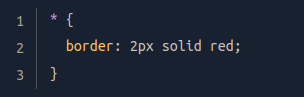
\includegraphics[width=\linewidth]{OdinProjectPics/borders.png}
		\caption{CSS code of a 2 pixel, solid red border}
		\label{border}
	\end{figure}

	%% Use float package to precisely place images
	\begin{figure}[H]
		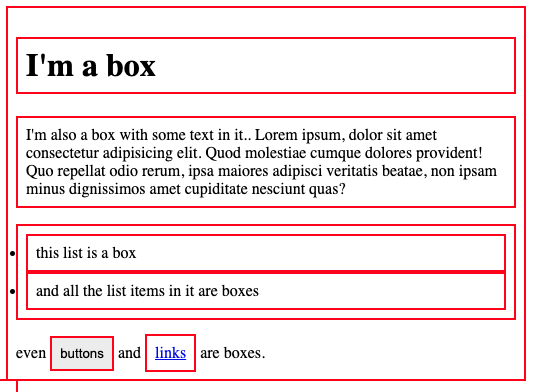
\includegraphics[width=\linewidth]{OdinProjectPics/boxes.png}
		\caption{HTML page of boxes with red borders}
		\label{boxes}
	\end{figure}

	\begin{figure}[H]
		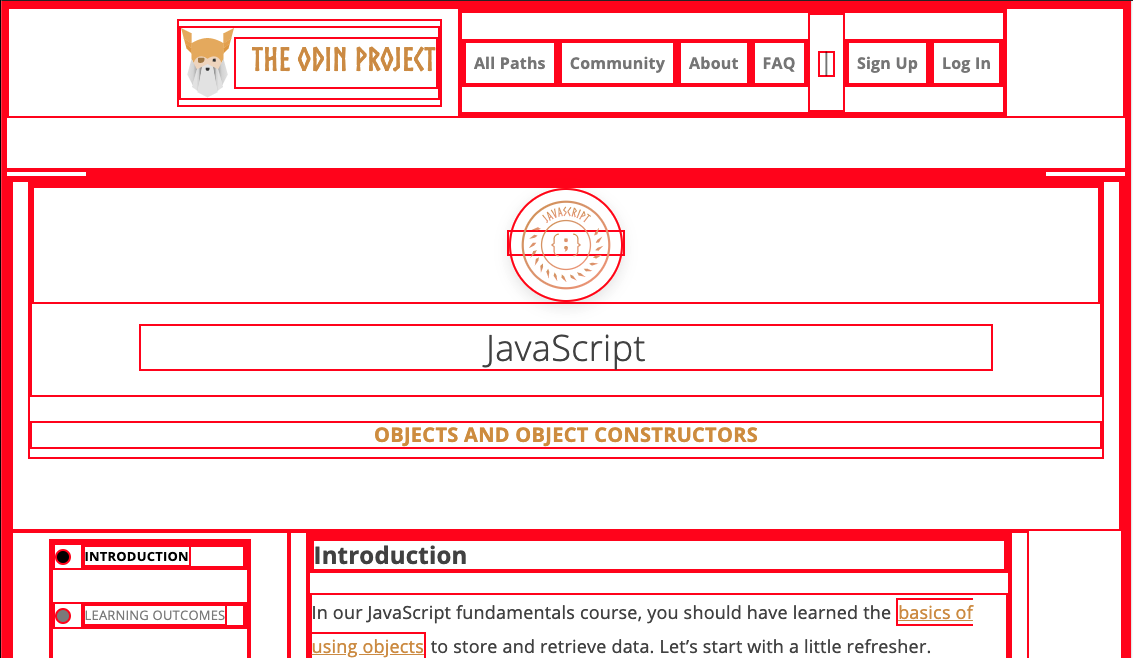
\includegraphics[width=\linewidth]{OdinProjectPics/odin-lined.png}
		\caption{Odin page with boxes}
		\label{Another example of boxes}
	\end{figure}

	In Figure 3, you may notice some circles but when it comes to layout, they fit more like rectangular boxes and not circles.
	Laying out a webpage \& positioning all its elements is deciding how you are going to nest \& stack these boxes.

	It can become quite complicted as there are many ways to manipuate the shape \& sizes of these boxes as well as the space between them, using 
	{\em padding}, {\em margin}, \& {\em border}. Note:

	\begin{itemize}
		\item {\bf Padding} increases the space between the edge of a box \& the content inside of it.
		\item {\bf Margin} increases the space between boxes
		\item {\bf border} adds space between the margin \& the padding
	\end{itemize}

	\begin{figure}[H]
		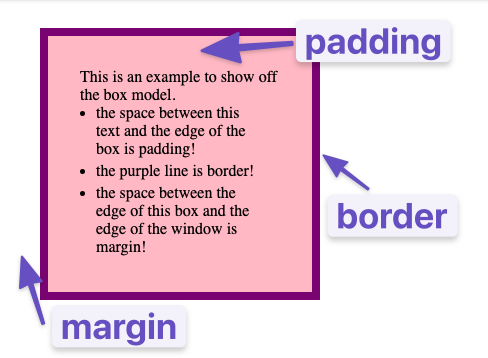
\includegraphics[width=\linewidth]{OdinProjectPics/box-model.png}
		\caption{Box model using padding, border, \& margin elements}
		\label{Box model}
	\end{figure}

	CSS has 2 main boxes:
	\begin{itemize}
		\item block boxes
		\item inline boxes
	\end{itemize}

\end{document}
